\documentclass[a4paper]{article}

\usepackage{xeCJK}
\usepackage{amsmath}
\usepackage{amssymb}
\usepackage[top=1in,bottom=1in,left=1.25in,right=1.25in]{geometry}
\usepackage{microtype}
\usepackage{siunitx}
\usepackage{enumerate}
\usepackage{indentfirst}
\usepackage{amsthm}
\usepackage{hyperref}

\linespread{1.5}
\setlength{\parskip}{0.4em} 

\setCJKmainfont[BoldFont=STHeiti,ItalicFont=STKaiti]{STSong}
\setCJKsansfont[BoldFont=STHeiti]{STXihei}
\setCJKmonofont{STFangsong}

\title{Mx* Compiler: Mid-term Report}
\author{郭文轩}
\date{\today}
\begin{document}
\maketitle

\section{心路历程}
现在已经完成了整个大作业的一小半。回头来看,前期走了不少弯路。

第一点是入门资料的选择。从零开始接触编译器,找到的资料主要是龙书虎书这样的大部头。翻开试读几页,算是了解了编译器开发的整体流程,但再往后的内容是深究细节的前端设计。就完成这项大作业而言,这些繁琐的事情交给工具效率更高,这些编译知识不如通过研究ANTLR等工具的文档学习来得具体形象,但当时也硬着头皮读了不少,最后于语义分析作罢。

后来找到了学长们留下的参考资料,包括书籍、设计思路等等,最开始拿着陈乐群学长的”big picture“pdf从更贴近实际的角度去了解我到底要写什么,怎么写,看了个大概,又看了看学长的代码框架,自己便开始动手。然而有一些很基本的问题都没有弄清楚,比如AST和parse tree的区别、符号表的设计等等,基本是不明所以地照抄。前面稀里糊涂地写,到语义分析的时候就发现寸步难行,觉得思路和代码一样混乱不堪。于是我又停下来,冷静思考了一段时间,找了些别的资料,重头开始。这次写的感觉思路流畅清晰,很清楚自己在做什么。只用了三四天的时间就把代码写好了,再结合数据修补了几处,挺顺利地通过了semantic test。

现在我最大的体会是:想清楚再动手,包括g4的语法设计。另一个心得是,ANTLR可以研究的东西不少,虽然我没有深入探索,但从文档中可以看出它的功能很强大,如果善用应该能进一步提高效率。当然,学习成本也需要考虑。

\section{遇到的问题}
说一说在具体的设计中几处模糊的地方。

首先是AST与ANTLR生成的parse tree。后者应该属于CST(concrete syntax tree),我要做的第一步是从这棵树自己建出一颗更灵活的AST,方便后面的检查、优化。

然后是``type node"和``type"与``symbol"。前者是AST上的一种节点,后者可以用《编程语言实现模式》一书的结构来解释.

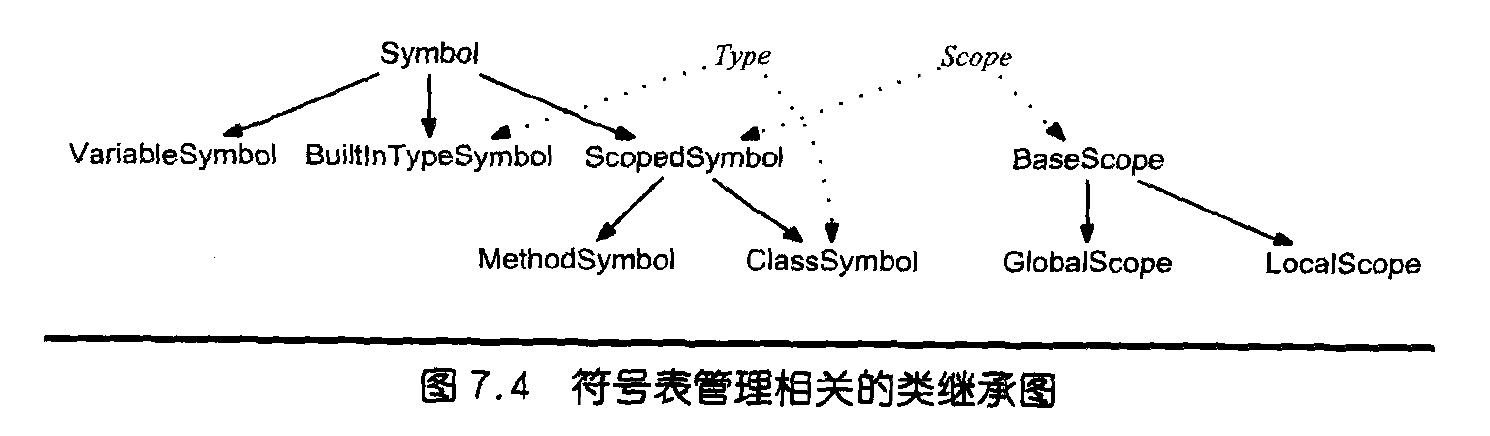
\includegraphics[width=5in]{symbol.png}

\section{建议}
OJ的使用说明要及时更新呀。

\section{推荐资料}
\href{https://github.com/abcdabcd987/compiler2016/blob/master/design/presentation.pdf}{design of Lequn Chen}

\href{https://book.douban.com/subject/4030327/}{Language Implementation Patterns}

\href{https://book.douban.com/subject/5288601/}{Engineering a Compiler}

\href{https://book.douban.com/subject/17912658/}{The Definitive ANTLR 4 Reference}

\end{document}